% Options for packages loaded elsewhere
\PassOptionsToPackage{unicode}{hyperref}
\PassOptionsToPackage{hyphens}{url}
%
\documentclass[
]{book}
\usepackage{lmodern}
\usepackage{amsmath}
\usepackage{ifxetex,ifluatex}
\ifnum 0\ifxetex 1\fi\ifluatex 1\fi=0 % if pdftex
  \usepackage[T1]{fontenc}
  \usepackage[utf8]{inputenc}
  \usepackage{textcomp} % provide euro and other symbols
  \usepackage{amssymb}
\else % if luatex or xetex
  \usepackage{unicode-math}
  \defaultfontfeatures{Scale=MatchLowercase}
  \defaultfontfeatures[\rmfamily]{Ligatures=TeX,Scale=1}
\fi
% Use upquote if available, for straight quotes in verbatim environments
\IfFileExists{upquote.sty}{\usepackage{upquote}}{}
\IfFileExists{microtype.sty}{% use microtype if available
  \usepackage[]{microtype}
  \UseMicrotypeSet[protrusion]{basicmath} % disable protrusion for tt fonts
}{}
\usepackage{xcolor}
\IfFileExists{xurl.sty}{\usepackage{xurl}}{} % add URL line breaks if available
\IfFileExists{bookmark.sty}{\usepackage{bookmark}}{\usepackage{hyperref}}
\hypersetup{
  pdftitle={Dragons Throughout Chinese Arts},
  pdfauthor={Dragon team},
  hidelinks,
  pdfcreator={LaTeX via pandoc}}
\urlstyle{same} % disable monospaced font for URLs
\usepackage{longtable,booktabs}
\usepackage{calc} % for calculating minipage widths
% Correct order of tables after \paragraph or \subparagraph
\usepackage{etoolbox}
\makeatletter
\patchcmd\longtable{\par}{\if@noskipsec\mbox{}\fi\par}{}{}
\makeatother
% Allow footnotes in longtable head/foot
\IfFileExists{footnotehyper.sty}{\usepackage{footnotehyper}}{\usepackage{footnote}}
\makesavenoteenv{longtable}
\usepackage{graphicx}
\makeatletter
\def\maxwidth{\ifdim\Gin@nat@width>\linewidth\linewidth\else\Gin@nat@width\fi}
\def\maxheight{\ifdim\Gin@nat@height>\textheight\textheight\else\Gin@nat@height\fi}
\makeatother
% Scale images if necessary, so that they will not overflow the page
% margins by default, and it is still possible to overwrite the defaults
% using explicit options in \includegraphics[width, height, ...]{}
\setkeys{Gin}{width=\maxwidth,height=\maxheight,keepaspectratio}
% Set default figure placement to htbp
\makeatletter
\def\fps@figure{htbp}
\makeatother
\setlength{\emergencystretch}{3em} % prevent overfull lines
\providecommand{\tightlist}{%
  \setlength{\itemsep}{0pt}\setlength{\parskip}{0pt}}
\setcounter{secnumdepth}{5}
\usepackage{booktabs}
\ifluatex
  \usepackage{selnolig}  % disable illegal ligatures
\fi
\usepackage[]{natbib}
\bibliographystyle{apalike}

\title{Dragons Throughout Chinese Arts}
\author{Dragon team}
\date{\texttt{December\ 18,\ 2020}}

\begin{document}
\maketitle

{
\setcounter{tocdepth}{1}
\tableofcontents
}
\hypertarget{motivation}{%
\chapter*{Motivation}\label{motivation}}
\addcontentsline{toc}{chapter}{Motivation}

Placeholder

\hypertarget{intro}{%
\chapter*{Introduction}\label{intro}}
\addcontentsline{toc}{chapter}{Introduction}

\hypertarget{ancient}{%
\chapter*{Dragon Art in Ancient China}\label{ancient}}
\addcontentsline{toc}{chapter}{Dragon Art in Ancient China}

Placeholder

\hypertarget{rise-of-dragon-sculptures-as-luxury-items--zhou__han}{%
\chapter{Rise of Dragon sculptures as luxury items \{-\#zhou\_\&\_han\}}\label{rise-of-dragon-sculptures-as-luxury-items--zhou__han}}

Placeholder

\hypertarget{tang}{%
\chapter*{Silk Road Influences}\label{tang}}
\addcontentsline{toc}{chapter}{Silk Road Influences}

\begin{center}\rule{0.5\linewidth}{0.5pt}\end{center}

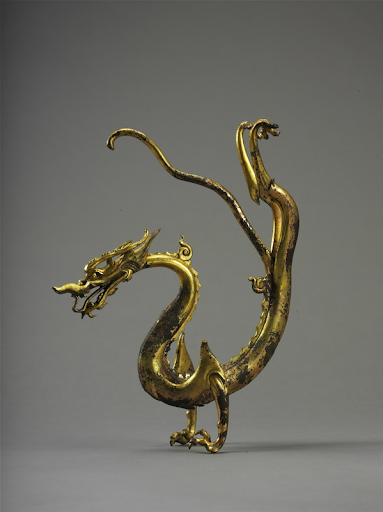
\includegraphics[width=1.2\textwidth,height=\textheight]{images/gilded_dragon.png}

\href{}{(Tang Dynasty). Mirror with Dragon, Bronze with Iron Core. Shaanxi History Museum, Xi'an.}

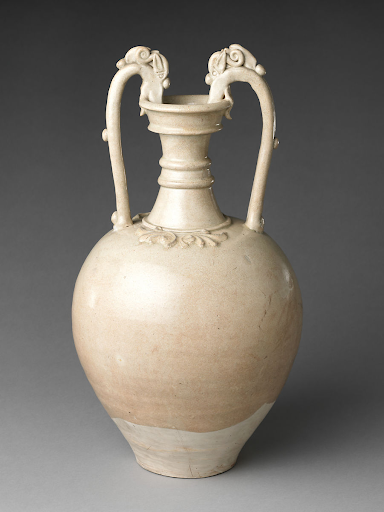
\includegraphics{images/jar.png}

\href{https://www.metmuseum.org/art/collection/search/45862}{(c.~7th century AD)., Tang Dynasty. Jar with Dragon-Headed Handles, Stoneware. The Metropolitan Museum, New York.}

\hypertarget{Dragon_Paintings}{%
\chapter*{Dragon Paintings in the Song and Yuan Dynasties}\label{Dragon_Paintings}}
\addcontentsline{toc}{chapter}{Dragon Paintings in the Song and Yuan Dynasties}

Placeholder

\hypertarget{the-emergence-of-dragon-paintings-in-the-song-dynasty}{%
\section*{The emergence of Dragon paintings in the Song Dynasty}\label{the-emergence-of-dragon-paintings-in-the-song-dynasty}}
\addcontentsline{toc}{section}{The emergence of Dragon paintings in the Song Dynasty}

\hypertarget{dragon-paintings-as-bearers-of-rain}{%
\section*{Dragon Paintings as Bearers of Rain}\label{dragon-paintings-as-bearers-of-rain}}
\addcontentsline{toc}{section}{Dragon Paintings as Bearers of Rain}

\hypertarget{ming}{%
\chapter*{Dragons as Political Symbols}\label{ming}}
\addcontentsline{toc}{chapter}{Dragons as Political Symbols}

Placeholder

A
\# References \{-\}

  \bibliography{book.bib,packages.bib}

\end{document}
